\documentclass[12pt, a4paper]{book}

\usepackage[utf8]{inputenc}
\usepackage[T1]{fontenc}
\usepackage[french]{babel}

\usepackage[hidelinks]{hyperref}  % sommaire cliquable
\usepackage{url}

% \usepackage[top=2cm, bottom=2cm, left=2cm, right=2cm]{geometry}
% \usepackage[top=3cm, bottom=3cm, left=3cm, right=3cm]{geometry}
\usepackage{bookman}
% \usepackage{newcent}


\usepackage{titletoc}  % écart chapitre numéro
\usepackage{blindtext}
\titlecontents{chapter}[1.5em]{\addvspace{1pc}\bfseries}{\contentslabel{5em}}{}
    {\titlerule*[0.3pc]{.}\contentspage}


\usepackage{pdfpages} %img full

\usepackage{afterpage}
\usepackage{xcolor}

% \usepackage{pythontex}
% \pyc{from tools import *}



\title{Harry Potter et les Méthodes de la Rationalité}
\author{Eliezer Yudkowsky}

\begin{document}
% \pagecolor{black}\afterpage{\nopagecolor}
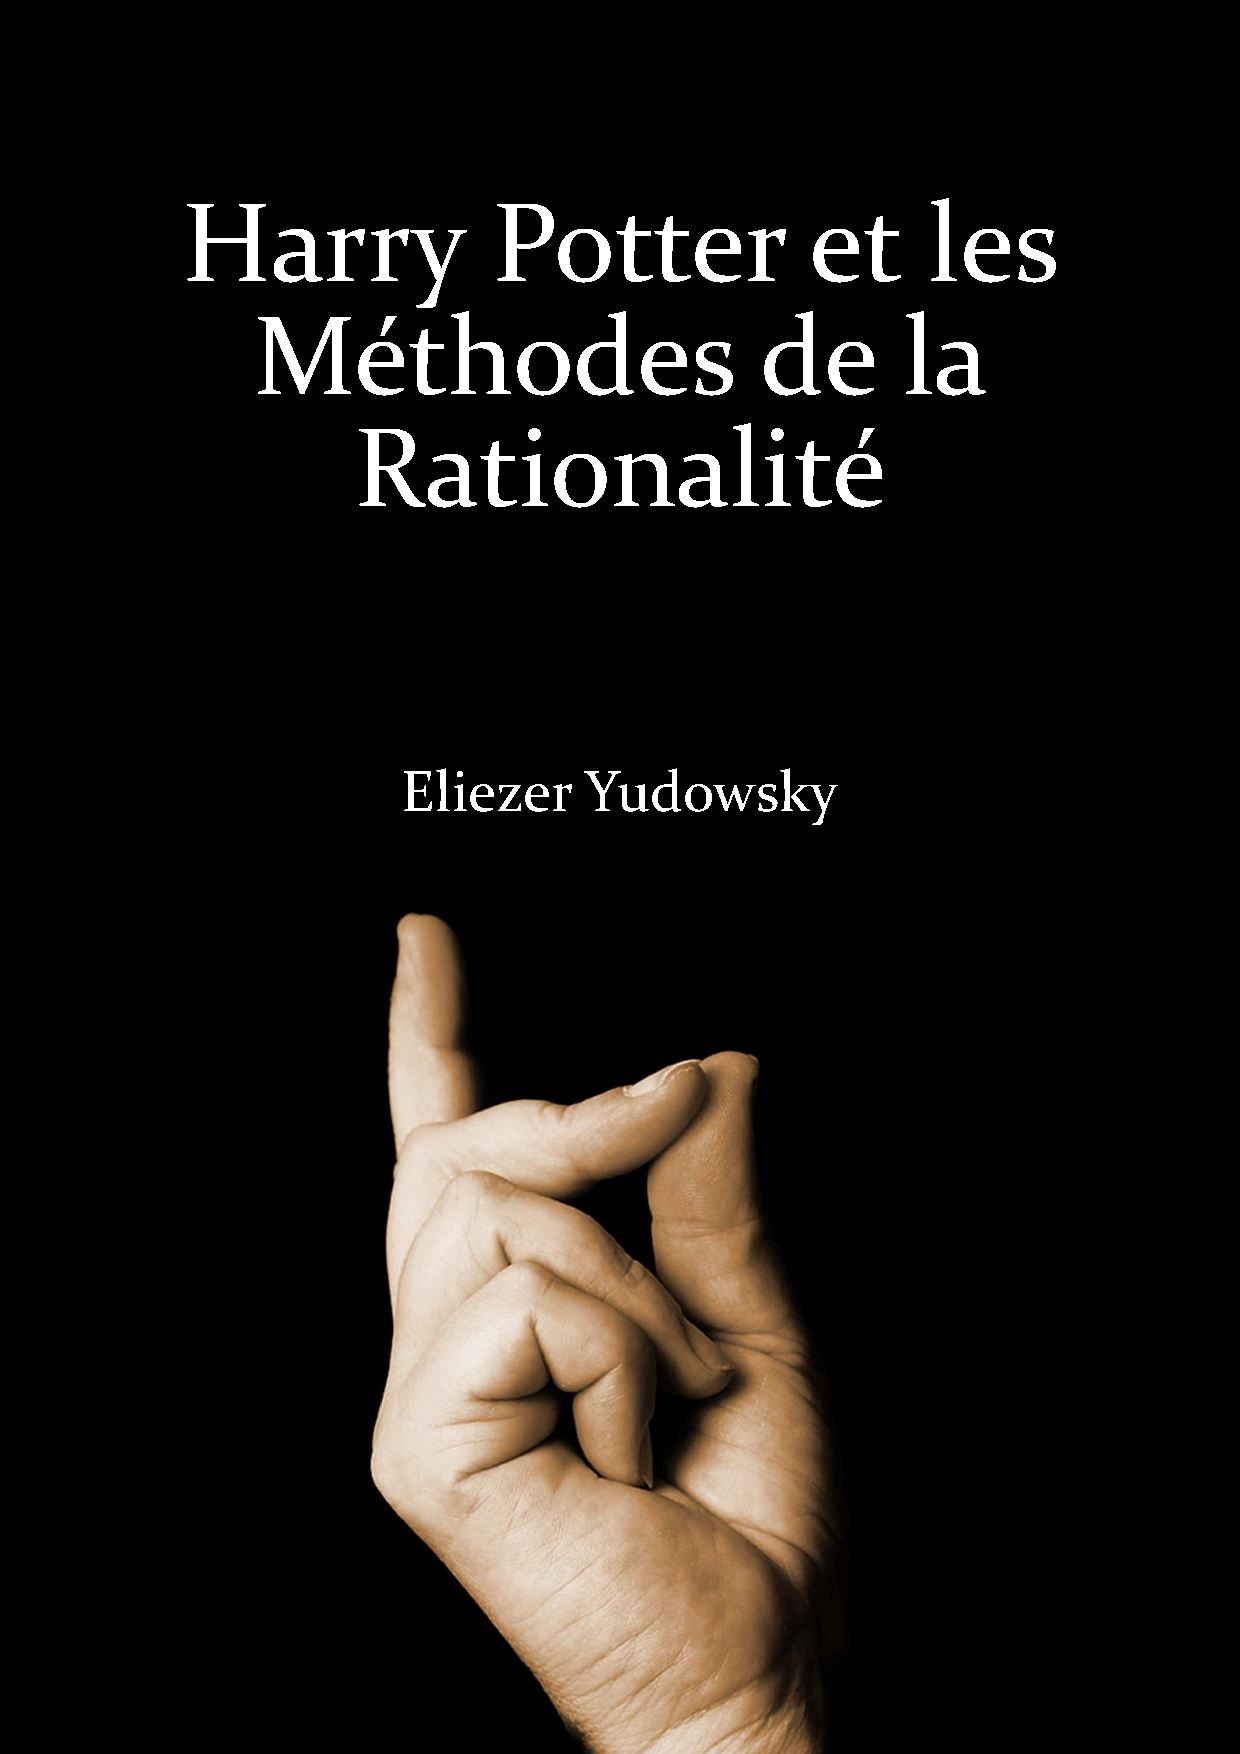
\includepdf{cover0.pdf}

Pour accéder à la version originale en anglais rendez-vous sur

\url{http://www.hpmor.com/}.

Cette traduction à été faîte par Adrien et est disponible ici :

\url{https://www.fanfiction.net/s/6910226/1/Harry-Potter-et-les-M%C3%A9thodes-de-la-Rationalit%C3%A9} 

Version du \today.

\tableofcontents


% \py{auto_include(range(1, 123))}

\input{chapter_list.tex}

\end{document}